\documentclass[paper=a4,11pt,german]{scrartcl} % default ist 10pt (zu klein)

\usepackage[utf8]{inputenc} % dokument muss dann auch als UTF-8 (ohne BOM) gespeichert werden
\usepackage[ngerman]{babel}

% schrfitauswahl
\usepackage[T1]{fontenc}
\usepackage[sc]{mathpazo}  % alternativ \usepackage{charter}
%\linespread{1.05}
\usepackage[scaled]{beramono}
\usepackage{multicol}
\setkomafont{sectioning}{\normalcolor\bfseries} % Ändert Überschriftschriftart (nun mit Serifen)

\usepackage{graphicx} 
% als letztes package (fuer funktionierende Link im und ausserhalb des Dokuments)
\usepackage[pdftex]{hyperref} 

% ggf. falsche Worttrennung hier korrigieren
\hyphenation{op-tical net-works semi-conduc-tor}

\begin{document}
%
% paper title
% can use linebreaks \\ within to get better formatting as desired
\title{Asymmetrische Kryptographie in Java}

\author{Norman Vetter\\
\textbf{Seminar "`Sichere verteilte Anwendungen mit Java"'}\\
Universität Potsdam\\
Wintersemester 2012/13}

\date{}

% make the title area
\maketitle

% Nicht bei einer Seminarausarbeitung. Da reicht die Zusammenfassung am Ende.
%
%\begin{abstract}
%Eine kurze Zusammenfassung.
%\end{abstract}
\newpage
\tableofcontents
\newpage
\section{Einleitung}
So sieht eine Section aus!

\section{Theoretische Grundlagen}

\subsection{Ziele}
Ein kryptographisches System dient zum verschlüsseln und entschlüsseln von Texten und anderen Daten, um deren Inhalt vor Dritten geheim zu halten. Genauer gibt ein Kryptosystem an wie ein Klartext in einen von Dritten nicht lesbaren Kryptotext umgewandelt werden kann. Und wie dieser Kryptotext später wieder in einen lesbaren Klartext transformiert wird. Anders als die Steganografie zielt die Kryptographie darauf ab lediglich den Inhalt einer Nachricht zu verschlüsseln, nicht aber deren Existenz zu verbergen. Die asymmetrische Kryptographie ist eines dieser kryptographischen Systeme.

\subsection{Asymmetrische Kryptographie}
Die asymmetrische Kryptographie wurde Mitte 1970 von Ralph Merkle sowie von Diffie und Hellmann entwickelt. Sie beruht auf der Idee zur Kommunikation zwischen 2 Instanzen ein Schlüsselpaar zu verwenden. Dieses Schlüsselpaar besteht aus dem privaten und dem öffentlichen Schlüssel. Zur Kommunikation muss im Vorhinein ein gegenseitiger Austausch des öffentlichen Schlüssels erfolgt sein, denn die zu schickende Nachricht ist vom Sender mit dem öffentlichen Schlüssel des Empfängers in einen Kryptotext um zu wandeln. Nach Empfang entschlüsselt der Empfänger nun die Nachricht mit seinem eigenen privaten Schüssel. Im Falle einer Antwort verschlüsselt der ehemalige Empfänger (nun Sender) seine Nachricht wieder mit dem öffentlichen Schlüssels seines Gegenüber. Welcher die Entschlüsselung erneut mit dem eigenen privaten Schlüssel durchführen muss. Somit ist während der Kommunikation kein erneuter Austausch eines sicheren Schlüssels notwendig und auch erneute Kommunikationen können mit den bereits vorhandenen Schlüsseln durchgeführt werden. Wichtig ist hierbei jedoch, dass die Sicherheit des privaten Schlüssels und die Authentizität des öffentlichen Schlüssels gewährleistet ist. Mehr dazu in den folgenden Kapiteln.
\newpage
\subsection{Grundlage asymmetrischer Systeme}
Im obigen Szenario haben wir gesehen wie ein grober Kommunikationsablauf zwischen Zwei Parteien aussieht. Dieses wird in folgender Grafik ( nach ~\cite{Eckert13} ) veranschaulicht:
\begin{figure}[htb]
	\centering
	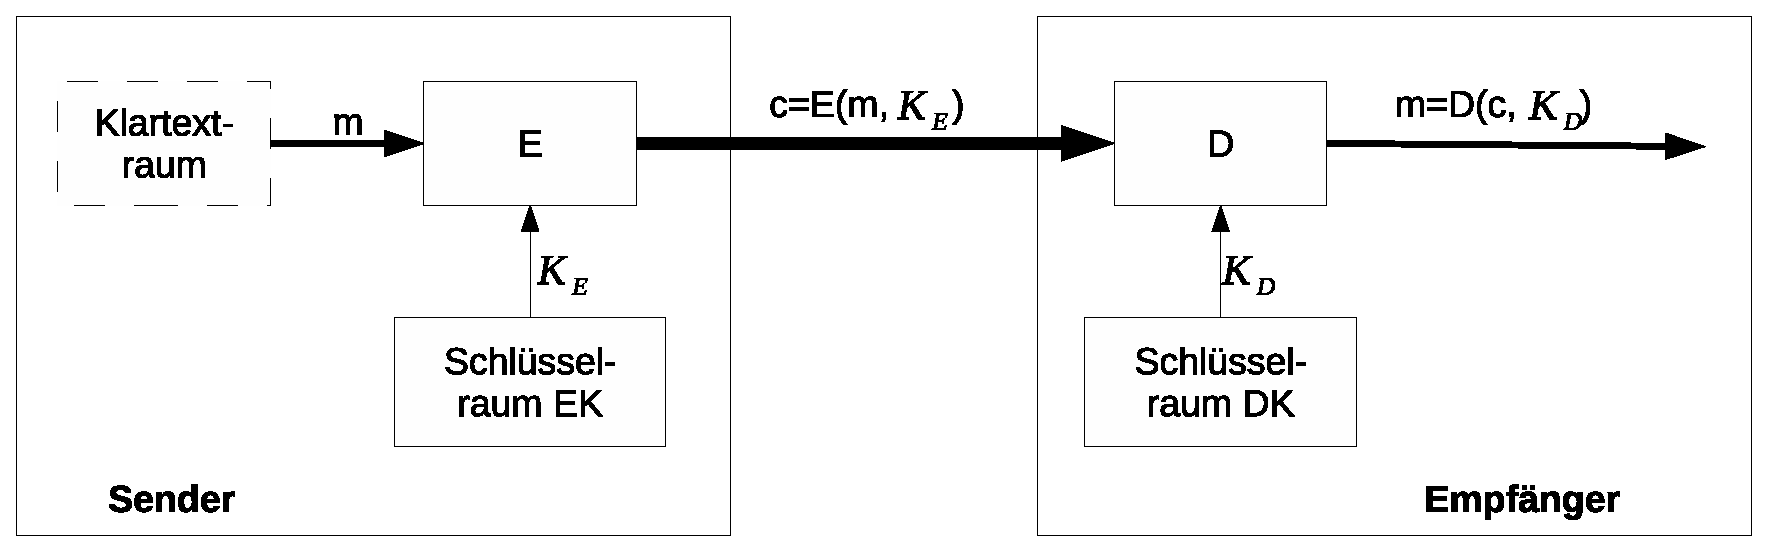
\includegraphics[width=\textwidth]{async.eps}
	\caption{Komponenten eines Kryptosystems}
	\label{fig:sim}
\end{figure}
\begin{multicols}{2}
\begin{enumerate}
\item Tupel \\($M,C,EK,DK,E,D$)
\item 2 endliche Alphabete \\($A_1,A_2$)
\item Menge von Klartexten \\($M \subseteq A^*_1\backslash\emptyset$)
\item Klartext \\($m \in M$)
\item Menge von Kryptotexten \\($C \subseteq A^*_2\backslash\emptyset$)
\item Kryptotext \\($c \in C$)
\item Verschlüsselungsschlüsselraum \\($EK\backslash\emptyset$)
\item Entschlüsselungsschlüsselraum\\($DK/\emptyset \\mit~ f:EK \rightarrow DK \\und~ f(K_E)=K_D)$
\item Verschlüsselungsverfahren \\($E :~ M x EK \rightarrow C$)
\item Entschlüsselungsverfahren \\($D :~ C x DK \rightarrow M$)
\item Es gilt: \\ $\forall m \in M : D(E(m,K_E),K_D) = m$
\end{enumerate}
\end{multicols}
Die Eigenschaft (11.) der Obigen Legende zeigt uns das Zusammenspielt unserer einzelnen Komponenten. Wird ein Klartext m mit einem Schlüssel $K_E \in EK$ durch ein kryptographisches Verfahren E in einen Kryptotext umgewandelt. So ist gegeben das dieser Kryptotext unter Verwendung des zu $K_E$ gehörigen Schlüssels $K_D \in DK$, und des kryptographischen Verfahrens D wieder in den ursprünglichen Klartext m umgewandelt werden kann. Damit dies gegeben ist muss unser asymmetrisches Kryptosystem einige wichtige Punkte erfüllen.
Es muss:
\newpage
\begin{itemize}
\item eine effiziente Möglichkeit zur Erzeugung von Schlüsselpaaren ($K_E,K_D$) geben.
\item garantiert sein das der Private ($K_D$) nicht effizient aus dem öffentlichen Schlüssel ($K_E$) gebildet werden kann.
\item möglich sein effizient zu Ver-. und Entschlüsseln.
\end{itemize}
Um dies zu erreichen nutzen wir Einwegfunktionen.
%\subsection{Anwendung asymmetrischer Systeme}
\subsubsection{Einwegfunktionen}
Einwegfunktionen sind besondere Funktionen ($f: X \rightarrow Y$) bei denen das Urbild ($X$) nicht unter vertretbarem, zeitlichem Aufwand aus dem Bild ($Y$) zu berechnen ist. Mathematische Probleme welche derartige Funktionen bilden sind unter Anderem das Faktorisierungproblem und der Diskrete Algorithmus. Es ist nicht bewiesen das die Umkehrung nicht möglich ist, jedoch Übersteigt die Komplexität der Berechnung unser heutiges Vermögen diese in einer vertretbaren Zeitspanne zu lösen.

Bei der Verwendung von normalen Einwegfunktionen in einem Kryptosystem wäre zwar die Sicherheit der Daten garantiert, jedoch stellt die Umkehrung selbst für autorisierte Personen ein unüberwindbares Hindernis dar. Wir benötigen zum Entschlüsseln unserer Daten eine Hintertür. Die so genannte Falltür. Einwegfunktionen mit Falltür bieten eine Identische Sicherheit wie normale Einwegfunktionen, und zudem die Option verschlüsselte Daten unter Kenntnis eines Geheimnisses (bei und der private oder öffentliche Schlüssel) zu entschlüsseln. Mathematische Probleme mit Falltür sind zum Beispiel die h-te Potenz modulo(n) oder der Zusammengesetzte modulo(n) (~\cite{Eckert13}). 
\subsubsection{RSA}
\subsubsection{Verschlüsselung und Endschlüsselung}
\subsubsection{Schlüsselmanagement}
\subsection{Hybride Kryptographie}


\section{Kryptographie mit Java}

\subsection{So wird zitiert}
Ein spannender Artikel ist~\cite{LSSZ08}. Lesenswert ist auch~\cite{oasa_mediawiki}

\section{Eine section mit eingebundener Abbildung}

In Abbildung~\ref{fig:sim} wird ... dargestellt. Es folgt eine
ausführliche Beschreibung:


\section{Zusammenfassung}
Zum Schluss bitte eine Zusammenfassung!

\bibliographystyle{alpha}
\bibliography{lit}

\end{document}
